\documentclass[12pt, eng, twoside, openany, final]{mgr}
% \documentclass[eng, printmode]{mgr}


% PREAMBULA


%% Language and font encodings
\usepackage[polish]{babel}
\usepackage[utf8x]{inputenc}
\usepackage[T1]{fontenc}

%% Sets page size and margins
\usepackage[a4paper,top=3cm,bottom=2cm,left=3cm,right=3cm,marginparwidth=1.75cm]{geometry}
%% \usepackage[a4paper, left=2.5cm, right=2.5cm, top=2.5cm, bottom=2.5cm, headsep=1.2cm]{geometry} -- Domski 

%% linki w spisie tresci, bibliografi
\usepackage[bookmarks=true,bookmarksnumbered=false,unicode=true,colorlinks=true,filecolor=black,linkcolor=black,urlcolor=black,citecolor=black]{hyperref}

\usepackage[colorinlistoftodos]{todonotes}


%OPEROWANIE NA OBRAZACH
\usepackage{graphicx}       % pakiet graficzny, umożliwiający m.in.
% import grafik w formacie eps
%\usepackage{epstopdf}		% pozwala na importowanie grafik w formacie eps
% przy użyciu pdflatex
\usepackage[update,prepend]{epstopdf}
\usepackage{rotating}       % pakiet umożliwiający obracanie rysunków
\usepackage{subfigure}      % pakiet umożliwiający tworzenie podrysunków
\usepackage{epic}           % pakiet umożliwiający rysowanie w środowisku latex
\usepackage{psfrag}         % pakiet umożliwiający podmianę łańcuchów znaków 
% w plikach eps
%\usepackage{curves}         % pakiet do wykreslania krzywych

%pakiety dodające dużo dodatkowych poleceń matematycznych
\usepackage{amsfonts}       % pakiet z rozmaitymi czcionkami matematycznymi
% \usepackage{amssymb}        % pakiet z rozmaitymi symbolami matematycznymi
\usepackage{amsmath}        % pakiet z rozmaitymi środowiskami matematycznymi

\usepackage{fp}             % pakiet z funkcjami operujacymi 
% na liczbach zmiennoprzecinkowych
\usepackage{calc}           % pakiet umożliwiający operacje arytmetyczne
% na tzw. licznikach (liczbach całkowitych)
\usepackage{leftidx}		% indeksy górne i dolne po lewej stronie

%definicje matematyczne
\providecommand{\abs}[1]{\lvert#1\rvert}
\providecommand{\norm}[1]{\lVert#1\rVert}

%pakiety wspomagające i poprawiające składanie tabel
\usepackage{supertabular}
\usepackage{array}
\usepackage{tabularx}
\usepackage{hhline}
\usepackage{longtable}		% wsparcie dla dlugich tabel
\usepackage{multicol}		% podzial strony na wiele kolumn

%pakiet do BibTex
\usepackage{cite}

\usepackage{url} %pakiet pozawalający na dodawanie adresów url w bibliografi

%pakiet wypisujący na marginesie etykiety równań i rysunków zdefiniowanych przez \label{}, chcąc wygenerować finalną wersję dokumentu wystarczy usunąć poniższą linię
%\usepackage{showlabels}

\usepackage{float}			% lepsza obsluga mechanizmow obiektow plywajacych
% wymuszenie wstawienia np. tabeli, obrazka w danym miejscu przez [H]

\usepackage{listings}       % pakiet dedykowany zrodlom programow
\usepackage{color}


\definecolor{dkgreen}{rgb}{0,0.6,0}
\definecolor{gray}{rgb}{0.5,0.5,0.5}
\definecolor{mauve}{rgb}{0.58,0,0.82}

\lstset{ %
	language=C++,                % the language of the code
	basicstyle=\scriptsize,           % the size of the fonts that are used for the code
	numbers=left,                   % where to put the line-numbers
	numberstyle=\tiny\color{gray},  % the style that is used for the line-numbers
	stepnumber=1,                   % the step between two line-numbers. If it's 1, each line 
	% will be numbered
	numbersep=5pt,                  % how far the line-numbers are from the code
	backgroundcolor=\color{white},      % choose the background color. You must add \usepackage{color}
	showspaces=false,               % show spaces adding particular underscores
	showstringspaces=false,         % underline spaces within strings
	showtabs=false,                 % show tabs within strings adding particular underscores
	%frame=single,                   % adds a frame around the code
	rulecolor=\color{black},        % if not set, the frame-color may be changed on line-breaks within not-black text (e.g. comments (green here))
	tabsize=2,                      % sets default tabsize to 2 spaces
	captionpos=b,                   % sets the caption-position to bottom
	breaklines=true,                % sets automatic line breaking
	breakatwhitespace=false,        % sets if automatic breaks should only happen at whitespace
	%title=\lstname,                   % show the filename of files included with \lstinputlisting;
	% also try caption instead of title
	keywordstyle=\color{blue},          % keyword style
	commentstyle=\color{dkgreen},       % comment style
	stringstyle=\color{mauve},         % string literal style
	escapeinside={\%*}{*)},            % if you want to add LaTeX within your code
	morekeywords={*,...},              % if you want to add more keywords to the set
	deletekeywords={...}              % if you want to delete keywords from the given language
}

%polish signs in lst code
\lstset{literate=%
	{ą}{{\k{a}}}1
	{ć}{{\'c}}1
	{ę}{{\k{e}}}1
	{ł}{{\l}}1
	{ń}{{\'n}}1
	{ó}{{\'o}}1
	{ś}{{\'s}}1
	{ż}{{\.z}}1
	{ź}{{\'z}}1
	{Ą}{{\k{A}}}1
	{Ć}{{\'C}}1
	{Ę}{{\k{E}}}1
	{Ł}{{\L}}1
	{Ń}{{\'N}}1
	{Ó}{{\'O}}1
	{Ś}{{\'S}}1
	{Ż}{{\.Z}}1
	{Ź}{{\'Z}}1
}

\usepackage{verbatim}       % pakiet dedykowany rozmaitym wydrukom tekstowym
\usepackage{ifthen}         % pakiet umożliwiający tworzenie prostych programów
% (m.in. zawiera instrukcje powtórzeniowe 
% i warunkowe)
\usepackage{upquote}		%normal quotations marks ' and `


% deklaracje wymagane przez pakiet theorem automatycznie ladowany w przypadku
% klasy dokumentu article
%
\newtheorem{Dn}{Definicja}[section]     % deklaracja srodowiska definicja
\newtheorem{La}[Dn]{Lemat}                % deklaracja srodowiska lemat
\newtheorem{Tm}[Dn]{Twierdzenie}          % deklaracja srodowiska twierdzenie
\newtheorem{Rk}[Dn]{Spostrze{\.z}enie}  % deklaracja srodowiska spostrzezenie
\newtheorem{Am}[Dn]{Algorytm}           % deklaracja srodowiska algorytm
\newtheorem{As}[Dn]{Za{\l}o{\.z}enie}   % deklaracja srodowiska zalozenie
\newtheorem{Pn}[Dn]{Propozycja}           % deklaracja srodowiska propozycja
\newtheorem{Py}[Dn]{W{\l}asno{\'s}{\'c}}  % deklaracja srodowiska wlasnosc
\newtheorem{Cy}[Dn]{Wniosek}              % deklaracja srodowiska wniosek
\newtheorem{Ee}[Dn]{Przyk{\l}ad}        % deklaracja srodowiska przyklad
\newtheorem{Ex}{{\'C}wiczenie}          % deklaracja srodowiska cwiczenie

\newtheorem{theorem}{Twierdzenie}[section] %nowe otoczenie do składania twierdzeń
%definicje własnych poleceń
\newcommand{\R}{I\!\!R} %symbol liczb rzeczywistych, działa tylko w trybie matematycznym

%helps to specify width of a column in table
%\begin{tabular}{|C{1cm}|c|c|c|c|c|c|c|c|c|c|}
%first column will have widht of 1cm
\newcolumntype{L}[1]{>{\raggedright\let\newline\\\arraybackslash\hspace{0pt}}m{#1}}
\newcolumntype{C}[1]{>{\centering\let\newline\\\arraybackslash\hspace{0pt}}m{#1}}
\newcolumntype{R}[1]{>{\raggedleft\let\newline\\\arraybackslash\hspace{0pt}}m{#1}}

\sloppy			%zawija bardzo długie linie

% \pagenumbering{gobble}% Remove page numbers (and reset to 1)
\usepackage{fancyhdr}
% \include{bibliografia}


% re-definiowane polecenie w celu przechowywania nazwiska autora, jego brak powoduje ostrzezenie (Warning) podczas przetwarzania.
\author{Piotr Szczpański} 

% re-definiowane polecenie w celu przechowywania polskiego tytułu pracy magisterskiej, jego brak powoduje ostrzezenie (Warning) podczas przetwarzania.
\title{Moduł sterownika oświetlenia LED} 


% polecenie zdefiniowane w celu przechowywania angielskiego tytułu pracy magisterskiej, jego brak powoduje ostrzezenie (Warning) podczas przetwarzania.
\engtitle{LED lighting controller module} 


% polecenie zdefiniowane w celu przechowywania danych osobowych prowadzacego prace, jego brak powoduje ostrzezenie (Warning) podczas przetwarzania.
\supervisor{dr inż. Antoni Izworski} 

% polecenie zdefiniowane w celu przechowywania danych osobowych opiekuna pracy. W przypadku gdy jest to ta sama osoba co \supervisor, nie nalezy uzywac tego polecenia. Jego brak usunie ze strony tytułowej zbedna informacje.
% \guardian{tytuł, Imie Nazwisko, jednostka} 


% polecenie zdefiniowane w celu przechowywania nazwy kierunku studiów, jego brak powoduje ostrzezenie (Warning) podczas przetwarzania.
\field{Automatyka i Robotyka (AIR)} 


% polecenie zdefiniowane w celu przechowywania nazwy specjalnosci studiów, jego brak powoduje ostrzezenie (Warning) podczas przetwarzania.
\specialisation{Robotyka (ARR)} 

% re-definiowane polecenie w celu przechowywania roku. Standardowo u dołu strony tytułowej wstawiany jest biezacy rok, uzycie tego polecenia pozwala wstawic dowolny rok.
\date{2018}
\usepackage{fancyhdr}

\begin{document}
\maketitle
\tableofcontents
\listoffigures
\newpage

\pagestyle{fancy}
\fancyhead{} 
\fancyfoot{} 
\lhead{Politechnika Wrocławska Wydział Elektroniki}
\rfoot{\thepage}
\lfoot{Szczepański P, Moduł sterownika oświetlenia LED}


\chapter{Wstęp}
\thispagestyle{fancy}
    \section{Wprowadzenie}
    W dzisejszczych czasach oświetlenie w naszych domach opórcz funkcji czysto praktycznej, ma również służyć jako dekoracja i stanowić integralną część wystroju. \\*
    Oświetlenie LED stanowi znaczącą część rynku elektroniki konsumenckiej i w ciągu kilkunastu lat wyparła prawie całkowicie z użytku codziennego wolframowe żarówki i lampy wyładowcze (potocznie zwane świetlówkami). Popularność technologii LED jest spowodowana głównie atrakcyjnymi cenami produktów i znacząco większą sprawnością elektryczną oraz co za tym idzie niższym zużyciem energii elektrycznej.
    
    \section{Cel i zakres pracy}
    Celem pracy jest stworzenie opisu powstawania, dokumentacji użytkownika i dokumentacji technicznej nowoczesnego sterownika oświetlenia LED opartego na platformie mikrokontrolerowej.
    
    Zakres pracy obejmuje opracowanie materiałów produkcyjnych, oprogramowania oraz fizycznego modelu. W szczególności zakres pracy obejmuje: 
    \begin{itemize}
        \item zaprojektowanie elektroniki, 
        \item zbudowanie modułu sterownika oświetlenia,
        \item stworzenie opiu i objaśnienia wykorzystanych technologii,
        \item wytworzenie oprogramowania oraz jego opisu funkcjonalnego,
        \item opracowanie dokumentacji technicznej modułu,
        \item opracowanie instrukcji obsługi modułu oraz dokumentacji dla użytkownika końcowego.
    \end{itemize}
%
\chapter{Założenia projektowe}
\thispagestyle{fancy}  
    Tworzony moduł będzie oferował użytkownikowi możliwość sterowania kolorami i jasnością trójkolorowego paska ledowego oraz sterwoanie dwoma wyjściami przekaźnikowymi. Użytkownik będzie komunikował się z modułem przez czterocalowy dotykowy wyświetlacz. Interfejs będzie udostępniał możliwość ręcznej zmiany stanów podłączonego oświetlenia, programowania własnych sekwencji zmiany kolorów paska LED i stanów wyjść przekaźnikowych oraz czasowego wywoływania zapisanych scen oświetleniowych.\\*
    Gotowy moduł sterowonika oświetlenia LED musi spełniać kryteria jakościowe, w szczególności:
    \begin{itemize}
        \item częstoliwość odświeżania generowango sygnału PWM sterującego pasek ledowy musi być na tyle wysoka, aby nie można było zaobserować migotania,
        
        \item graficzny interfejs użytkownika powinien być przejżysty, intuicyjny w obsłudze oraz na tyle responsywny, żeby
        obsługa modułu była komfortowa,
        
        \item moduł musi działać w ciągłości, tzn. konfiguracja wbudowanego systemu operacyjnego musi zabezpieczać sytuacje
        krytycznych błędów czasu działania, między innymi takich jak: desynchronizacja systemowego zegara, wyłączenie aplikacji interfejsu graficznego
    \end{itemize}
%
\chapter{Opis wykorzystanych technologii}
\thispagestyle{fancy}
    \section{Raspberry Pi}
    Raspberry Pi jest serią jednopłytkowych komputerów opartych na rdzeniach ARM. Pod nazwą Raspberry Pi kryje się również olbżymia społeczność rozwijająca oprogomowanie, tworząca biblioteki i materiały edukacyjne.
    W projekcie wykorzystano model \emph{Raspberry Pi Zero W V1.3} oparty na procesorze  \emph{Broadcom BCM2835 ARM11}. Moduł wyposażony jest m.in. w 512MB pamięci RAM, moduł WiFi, moduł Bluetooth, port miniHDMI. Z uwagi na  duże możliwości techniczne oraz niską cenę, modułu ten jest powszechnie wykorzystywany przy prototypowaniu urządzeń elektronicznych IoT.
    
    \section{Język C++}
    Język C++ powstawł w roku 1979 stworzony przez Bjarne Stroustrup'a jako rozszerzenie języka, od tego czasu C++ doczekał się kilku standardów i od 2011 roku co 3 lata wydawana jest jego nowa wersja. C++ osiągną olbrzymią popularność dzięki swojej uniwersalności. W komercjnych zastosowaniach przy tworzeniu oprogramowania na wbudowane systemy wbudowana często wypiera używanie czystego języka~C. C++ pozwala na tworzenie kodu zarówno nisko jak i wyskopoziomowego. Kod może być zarówno zorientowany obiektowo jak również czysto procedulany. 
    enkapsulacja
    polimorfizm
    biblioteki
    boost
    
    
    \newpage
    \section{Biblioteka QT i QML}
    QT jest zestawem bibliotek, których głównym celem jest tworzenie interfejsów graficznych aplikacji komputerowych. Ponadto QT dostarcza wiele narzędzi programistycznych pomagających rozwijać oprogramowanie. Oprócz zastosowań komputerowych QT daje możliwości tworzenia aplikacji na urządzenia wbudowane i jest powszechnie używane przez takie firmy jak: LG, Mercedes-Benz.
 
%
\chapter{Dokumentacja użytkownika}
\thispagestyle{fancy}
    \section{Podłączanie zasilania i urządzeń wykonawczych}
    Moduł zasilany jest napięciem 12V i nie posiada zabezpieczenia przeciw odwrotnej polaryzacji zasilania. więc błędne podłączenie zasilacza może uszkodzić sterownik. \\*
    Maksymalna moc oświelenia podłączonego do wyjść wynosi:
    \begin{itemize}
        \item sumarycznie dla wyjść sterownika paska led : 00W, czyli dla każdego kanału 00W,
        \item dla każdego z wyjść przekaźnikowych : 100 W
    \end{itemize}
    Instalator musi pamiętać, że podłączone obciążenie nie może przekraczać maksymalnej mocy zasilacza ponadto maksymalny prąd zasilacz powinien wynosić przynajmnej 750mA, więcej niż potrzebuje tego obicążenie, gdyż należy doliczyć zapotrzebowanie Raspberry Pi z wyświetlaczem. Podane 750mA jest wartością bezpieczną i nie znaczy to, że moduł pobiera w trakcie swojego działania taki prąd. \\*
    Zasilacz należy podłączyć do złącza \emph{J5}, wyjścia przkaźnikowe są oznaczone symbolami \emph{J3}, \emph{J4}, a sterownik paska ledowego \emph{J1J2}. Sposób podłączenie paska led jest oznaczony bezpośrednio na płytce. 
        \begin{figure}[H]
        \begin{center}
            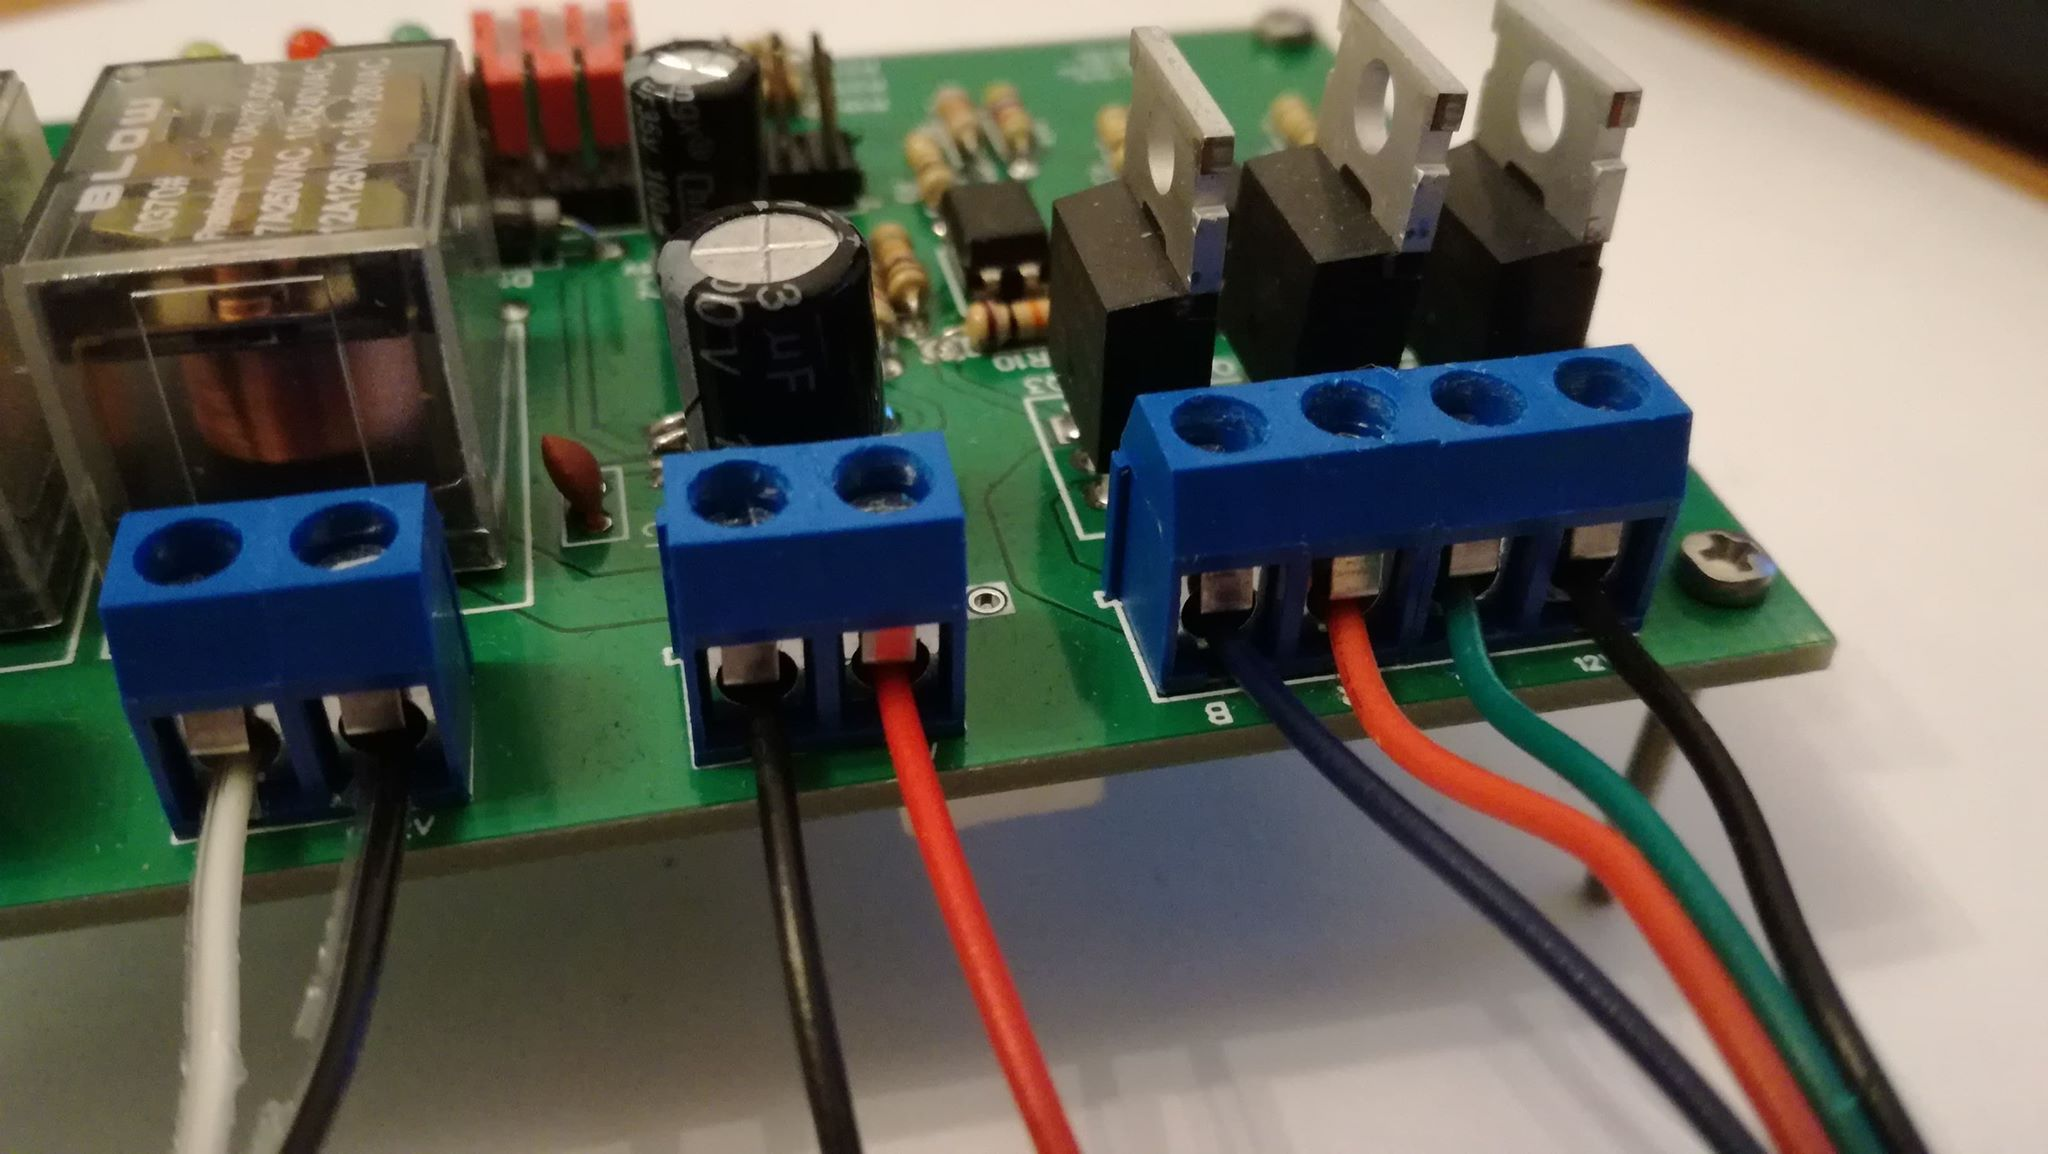
\includegraphics[width=0.65\textwidth]{podlaczone.jpg}
            \caption{Przykład podłączenia zasilania, paska led oraz żarówki led}
        \end{center}
        \end{figure}
    
    \section{Opis interfejsu graficznego}
    \section{Konfiguracja funkcji}
        \subsection{Tworzenie scen}
        \subsection{Tworzenie animacji}
        \subsection{Tworzenie zdarzeń czasowych}
%
\chapter{Dokumentacja serwisowa}
\thispagestyle{fancy}
    \section{Typowe wykorzystanie}
    Przeznaczeniem modułu jest wykorzystanie w pomieszczeniu użytkowym, do sterowania intensywnością świecenia poszczególnych kolorów paska ledowego oraz do przełączania dwóch dwunastowoltowych wyjść przekaźnikowych. Wyjścia przekaźnikowe zostały umieszczone w projekcie aby pozwolić użytkownikowi podłączyć i sterować np.: stanem jednokolorowego paska LED, stanem żarówki LED lub zewnętrznym przekaźnikiem bądź stycznikiem. Maksymalne parametry elektryczne określone są w sekcji \emph{5.2.1 Elektornika wykonawcza}.
    \newpage
    
    \section{Budowa modułu}
    Sterownik składa się z zaprojektowanej płytki z elektroniką wykonawczą i stabilizatorem napięcia, połączonej wielożyłowym kablem z modułem \emph{Raspberry Pi}, do którego, za pomocą listwy goldpin, podłączony jest wyświetlacz dotykowy.
        \begin{figure}[H]
        \begin{center}
            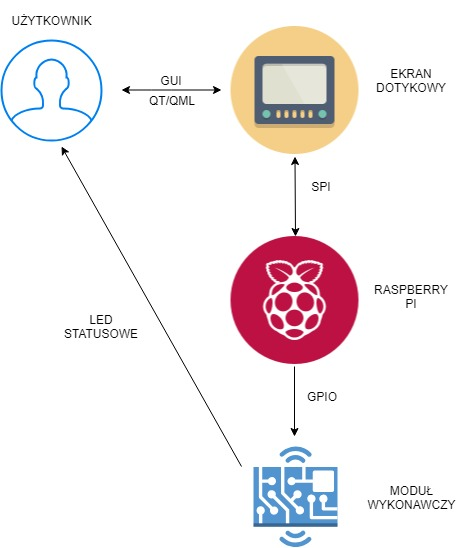
\includegraphics[width=0.4\textwidth]{diagram.jpg}
            \caption{Schemat ideowy modułu}
        \end{center}
        \end{figure}
        
       
        \begin{figure}[!h]
        	\centering
        	\begin{minipage}[t]{5cm}
        		\centering
        		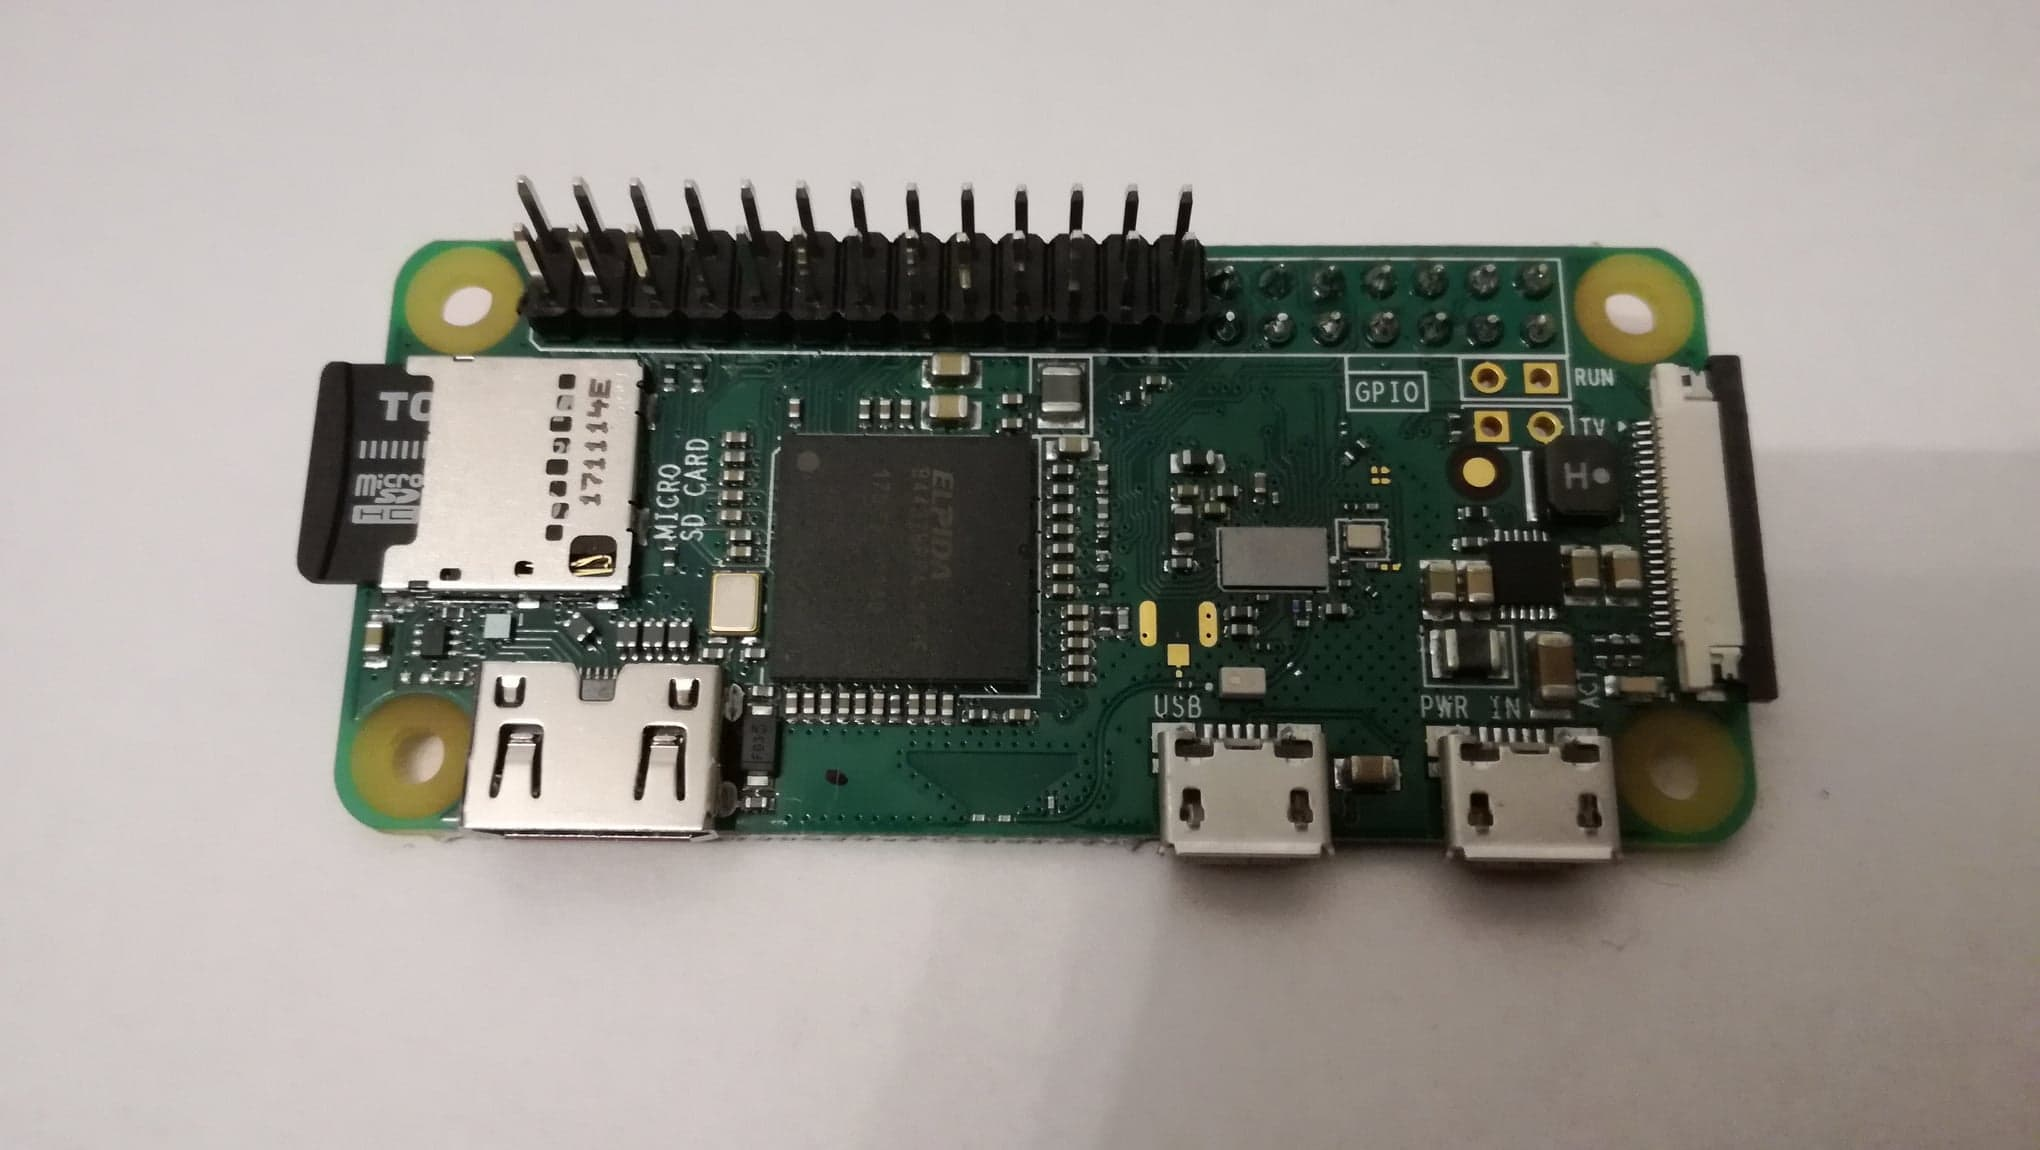
\includegraphics[scale=0.1]{rpi_goldpin.jpg}
        		\caption{Raspberry Pi z przylutowanymi złączami goldpin} \label{fig:rpi1} 
        	\end{minipage}
        	\hspace{3cm}
        	\begin{minipage}[t]{5cm}
        		\centering
        		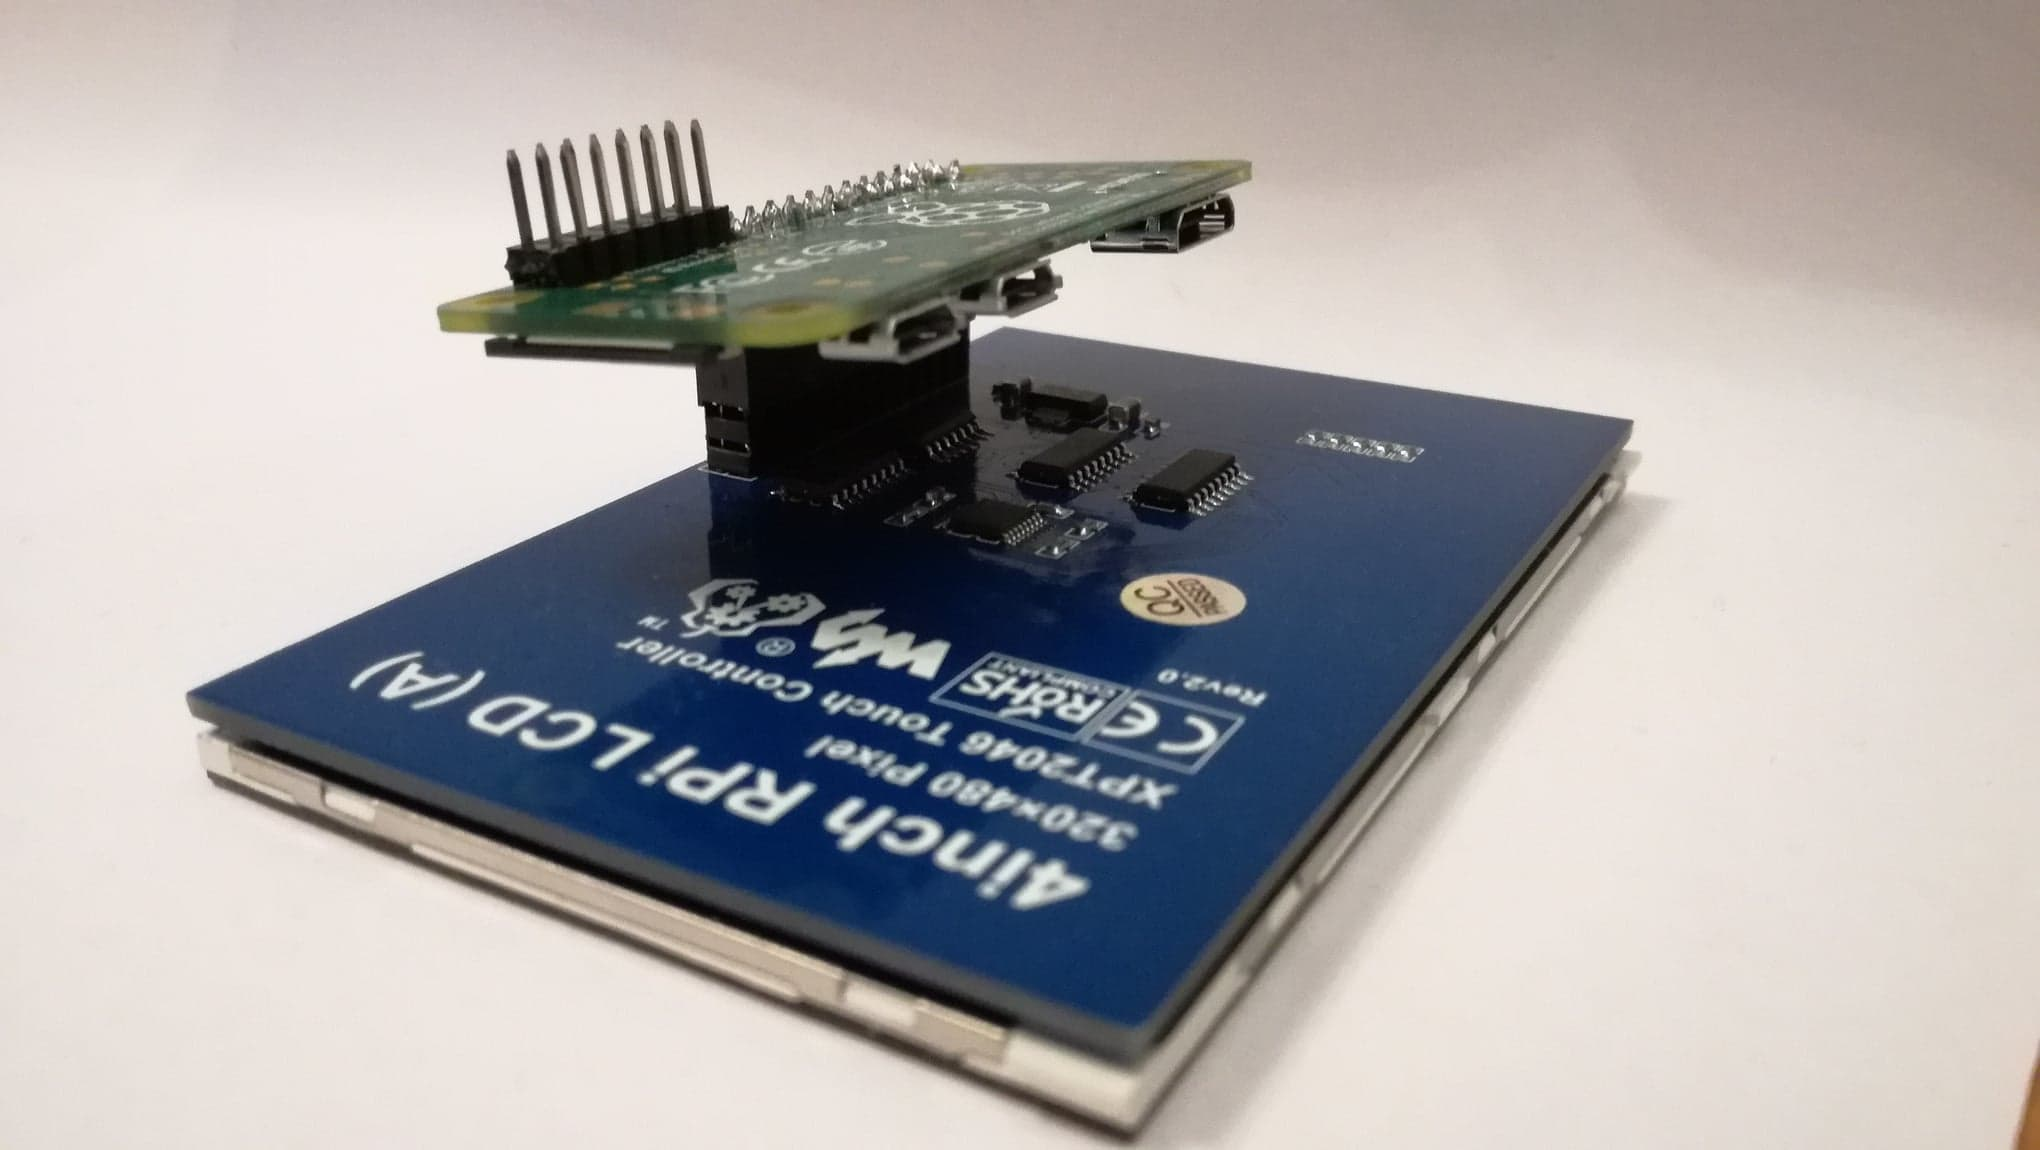
\includegraphics[scale=0.1]{rpi_lcd.jpg}
        		\caption{Połączenie Raspberry Pi z wyswietlaczem dotykowym} \label{fig:rpi_lcd} 
        	\end{minipage}
        \end{figure}
        Dzięki takiej budowie elementy wydzielające ciepło, takie jak tranzysory i procesor, mogą być od siebie oddalone. 
        \newpage
        
        \begin{figure}[H]
            \begin{center}
            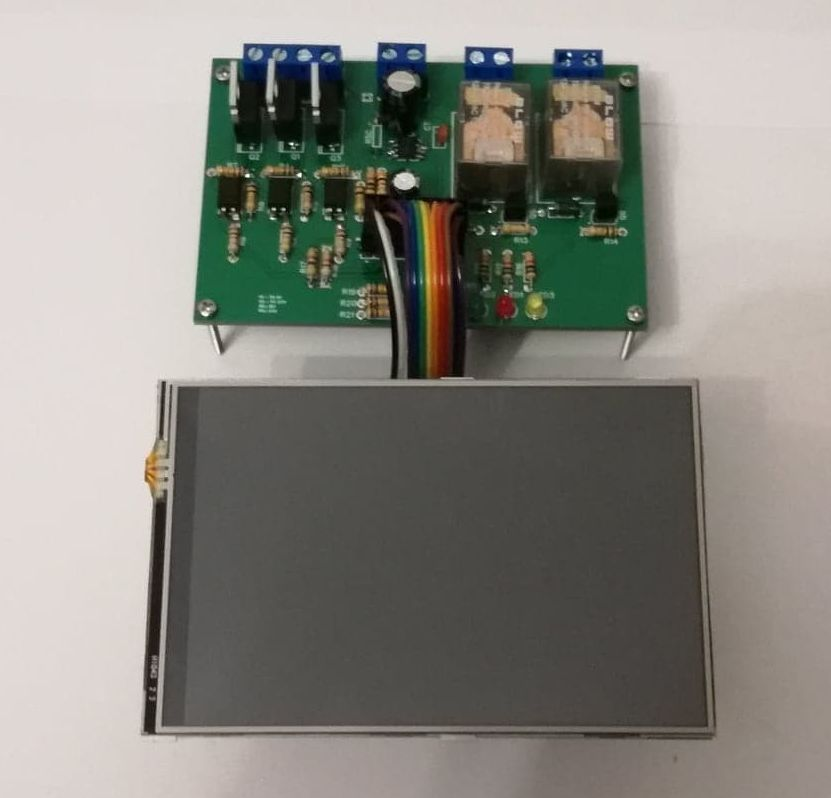
\includegraphics[width=0.6\textwidth]{poloczona_zoom.jpg}
            \caption{Moduł wykonawczy połączony z Rapsberry Pi}
            \end{center}
        \end{figure}
        
        \newpage
        \subsection{Elektronika wykonawcza}
            \subsubsection{Sterownik paska LED}
                Protoypowanie modułu rozpoczęto od budowy sterownika paska ledowego, który sterowany był z prostego 8-bitowego mikrokontorlera \emph{Atmega 168P}. 
                Sterownik składa się z trzech identycznych kanałów, osobnego dla każdego koloru paska. 
                \begin{figure}[H]
                \begin{center}
                    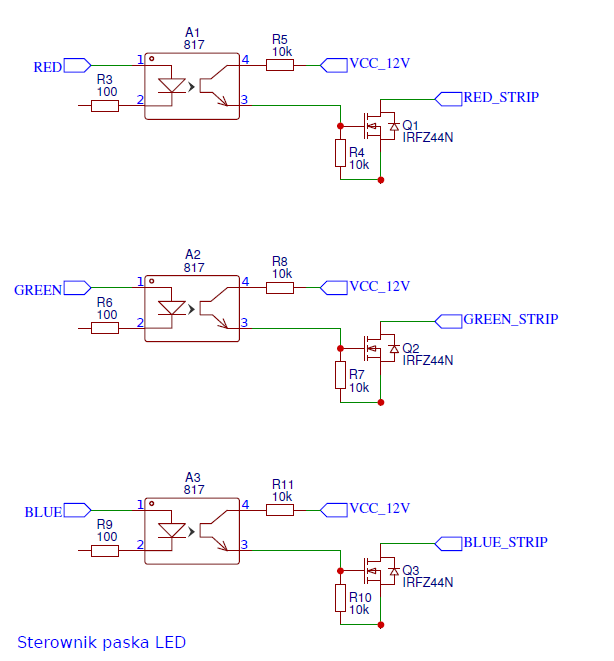
\includegraphics[width=0.45\textwidth]{sterownik.png}
                    \caption{Schemat trzykanałowego sterownika paska LED}
                \end{center}
                \end{figure}
                Elementem wykonawczym są tranzystory MOSFET (ang. Metal-Oxide Semiconductor Field-Effect Transistor), oznaczone na schemacie symbolami \emph{Q1}, \emph{Q2}, \emph{Q3}. Po podaniu między złącza bramka(ang. gate) i źródło(ang. source), określonego w nocie katalogowej, napięcia, tranzysor zaczyna przewodzić między złączami dren(ang. drain)-źródło. Należy pamiętać, żę między drenem, a źródłem występuje rezystancja określona w nocie katalogowej symbolem Rds(on). Jest to ważny parametr, ponieważ ma on wpływ na ilość energii, która zostanie wytracona w formie ciepła, a co za tym idzie maksymalny prąd jaki tranzysor może przewodzić bez przegrzewania~się.
        
                \newpage
        
            \subsubsection{Wyjścia przekaźnikowe}
            Moduł wyposażono również w dwa wyjścia przekaźnikowe pozwalające użytkownikowi na sterowanie stanem m.in. takich peryferiów jak: jednokolorowy pasek ledowy, żarówka led. W projekcie wykorzystano przekaźniki \emph{BLOW JQC-3F 12VDC}, dopuszają one przełączanie 10A prądu stałego przy 12V.
            Moc cewki wybranych przekaźników wynosi 0.45W, więc w celu ich sterowania należało użyć tranzystor MOSFET. Niezbędnym elementem obwodu sterownikia trnazystorowego przekaźników jest dioda, \emph{D3}, \emph{D4}, zabezpieczająca tranzystor przed energią znajdującą się w cewce przekaźnika, który zostaje z niej wydalona pod wpływem zapadania się pola magnetycznego.
                \begin{figure}[H]
                \begin{center}
                    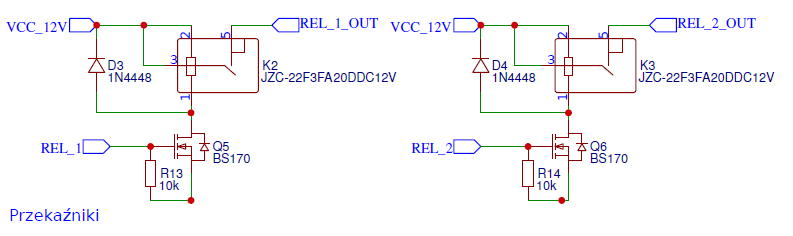
\includegraphics[width=0.75\textwidth]{przekazniki.png}
                    \caption{Schemat wyjść przekaźnikowych}
                \end{center}
                \end{figure}
        \subsection{Przetwornica napięcia}
        Na płytce znajudje się również przetwornica napięcia, która służy zasileniu Raspberry Pi Zero. Zdecydowano się na wykorzystanie \emph{ON Semiconductor MC34063A} z uwagi na dużą dostępność, niską cenę oraz łatwość użycia. Moduły MC34063 pracują w zakresie napięcia wejściowego od 3V do 40V i mogą być skonfigurowane w trybie obniżania, podwyższania lub odwracania napięcia. Maksymalny prąd wyjściowy to 1.5A, jest to wartość przekraczająca potrzeby przy zasilaniu większości mikroprocesorów. Sterowanie parametrami układu DC-DC odbywa się przez dobór wartości elementów pasywnych. Nota katalogowa układu dostarcza potrzebne w wzory potrzebne do obliczenia wartości elementów.
                \begin{figure}[H]
                \begin{center}
                    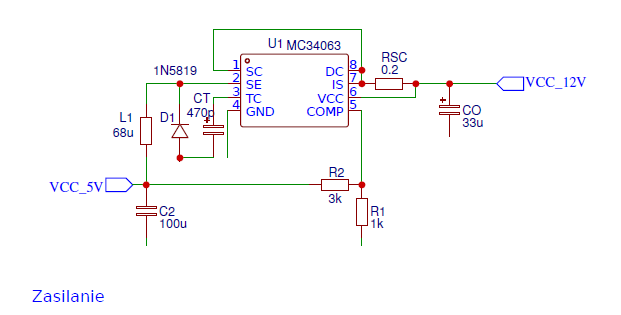
\includegraphics[width=0.75\textwidth]{psu.png}
                    \caption{Schemat przetwornicy napięć}
                \end{center}
                \end{figure}
                
        Parametry wyjściowe układu wynoszą:
        \begin{itemize}
            \item Napięcie wejściowe : 12V
            \item Napięcie wyjściowe : 5V
            \item Częstotliwość      : Hz 
            \item Wahania napięcia wyjściowego : Vpp 
        \end{itemize}
                
        \subsection{Elektronika dodatkowa}
        Na płytce umieszczono również elementy służące wyłącznie weryfikacji poprawności działania układu.
        
        \subsubsection{Przełącznik trybów pracy}
            \begin{figure}[H]
            \begin{center}
                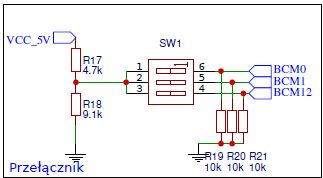
\includegraphics[width=0.4\textwidth]{przelacznik.jpg}
                \caption{Schemat przełącznika trybów pracy}
            \end{center}
            \end{figure}
        W celach zmiany trybów diagnostycznych na płytce znajduje się potrójny przełącznik suwakowy. Z uwagi na 3.3V poziom logiczny Raspberry Pi i fakt, że na płytce znajduje się jednynie przetwornica napięcia o 5-cio V wyjściu należało stowrzyć dzielnik napięciowy tworzony z rezystorów R17 i R18. Rezystory R19, R20, R21 są rezystorami podciągającymi.  
        \subsubsection{Diody sygnalizujące stan pracy}
            \begin{figure}[H]
            \begin{center}
                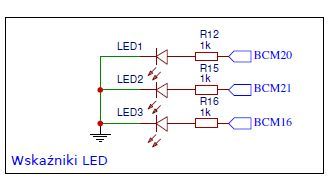
\includegraphics[width=0.4\textwidth]{wskaznik.jpg}
                \caption{Schemat diod sygnalizacyjnych} 
            \end{center}
            \end{figure}
        Moduł posiada 3 diody sygnalizacyjne służące do informowania użytkownika o błędach lub mogące być wykorzystane przy sprawdzaniu modułu. Rezystory R12, R15, R16 dobrano tak aby intesywność świecenia diod nie sprawawiała dyskomfortu serwisantowi badającemu sterownik.
        
        \subsection{Wyświetlacz dotykowy}
            \begin{figure}[H]
            \begin{center}
                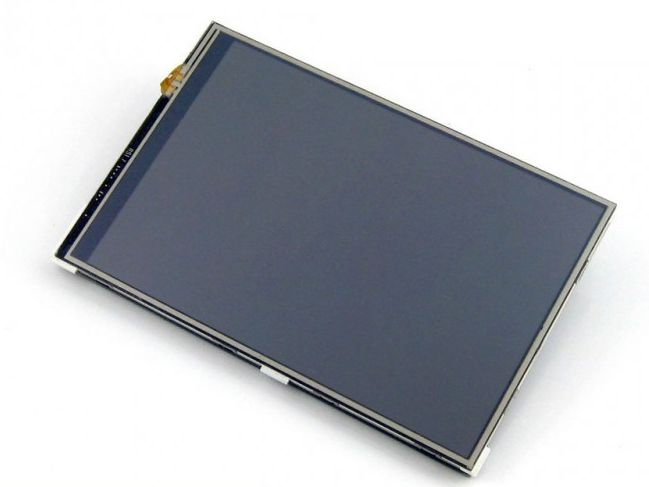
\includegraphics[width=0.6\textwidth]{wyswietlacz.jpg}
                \caption{Wyświetlacz dotykowy używany w module} 
            \end{center}
            \end{figure}
            tft 4cale spi waveshare połączenie z rpi patent
            W projekcie zdecydowano się na użycie gotowego modułu wyświetlacza dotykowego 
            \emph{Waveshare}. Jego rozmiar to 95 x 61 mm i posiada rozdzielczość 320x480 pikseli. Z uwagi na te dwie własności, graficzny interfejs użytkownika został zaprojektowany tak aby  

        
        \subsection{Płytka drukowana}
            Po zakończonym etapie prototypowania poszczególnych partii, elementy te zostały połączone w jeden schemat, na podstawie którego zaprojektowano płytkę drukowaną (PCB). 
            Płytka ma wymiary 90x62mm, jest 
            Seria prototypowa płytek została 
            
    \section{Instrukcja montażu}
    Montaż układu powinno rozpocząć się od wizualnego sprawdzenia poprawności wykonania płytki drukowanej, ważnym jest sprawdzenie czy wszystkie punkty lutownicze są poprawnie pokryte i czy ścieżki nie wyglądają na uszkodzone, np. w transporcie.
    Pierwszym krokiem jest przylutowaie przetwornicy napięć, ponieważ jest to najmniejszy element i jej montaż może być później utrudniony przez sąsiadujące elementy. Dalej należy przylutować transoptory \emph{A1}, \emph{A2}, \emph{A3}.  Następnie w dowolnej kolejności można przylutować: rezystory \emph{R1} do \emph{R21}, kondensatory \emph{C0}, \emph{Ct}, \emph{C2}, diody \emph{D1}, \emph{D3}, \emph{D4}, tranzystory \emph{Q1}, \emph{Q2}, \emph{Q3}, \emph{Q5}, \emph{Q6}, diody led \emph{LED1}, \emph{LED2}, \emph{LED3}. Po wykonaniu tych czynności należy przylutować złącze \emph{JP1}, przełącznik suwakowy \emph{SW1}, złącza ARK \emph{J1} - \emph{J5}. Ostatnimi elementami na górnej warstwie są przekaźniki \emph{K2}, \emph{K3}. Na dolej warstwie płytki powinna znaleźć się cewka \emph{L1} i rezystor \emph{RSC}, tak jak jest to widoczne na \ref{fig:pcb_dol}. \\*
    Złącza goldpin na Raspberry Pi powinne zostać polutowane tak aby piny od 27 do 40 były skierowane w kierunku przeciwnmy do mikroprocesora na płyce (patrz \ref{fig:rpi1}), pozostałe odwrotnie. 
            \begin{figure}[H]
            \begin{center}
                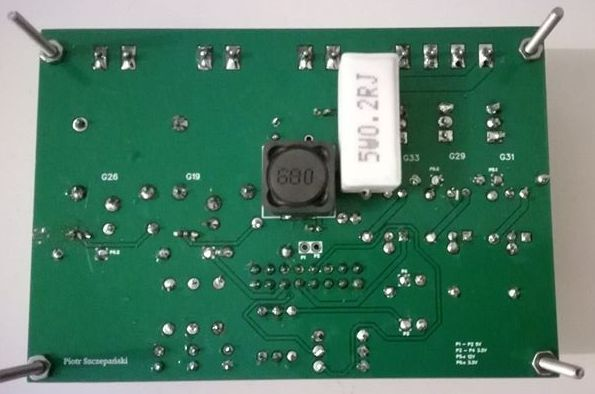
\includegraphics[width=0.5\textwidth]{dol.jpg}
                \caption{Dolna warstwa płytki} \label{fig:pcb_dol} 
            \end{center}
            \end{figure}
    Montaż wyświetlacza dotykowego do płytki Raspberry Pi odbywa się przez wsunięciego w złącze goldpin, poprawny instalacja widoczna jest na \ref{fig:rpi_lcd}. Komunikacja płytki sterującej z płytką wykonawczą odbywa się przez 16-sto żyłowy kabel, który od strony płytki wykonawczej powinnien być zakończony damski złączem 2x8 goldpin, a na drugim końcu złączem 2x7 oraz dwoma przewodami, które muszą zostać przylutowane do pinów 3 (5V) i 4 (GND) na Raspberry Pi. 

    \newpage
    \section{Sprawdzanie modułu}
            Płytka i opis znajdujący się na niej został zaprojektowany tak, aby w łatwy sposób można było sprawdzić poprawność działania modułu. 
            
            \subsubsection{Sprawdzanie poprawności działania samego modułu wykonawczego}
            Dolna strona PCB zawiera dwa rodzaje oznaczeń, które służą do sprawdzenie poprawności działania elektroniki płytki:
            \begin{itemize}
                \item oznaczaczenia \emph{G*} informujące do którego pinu mikroprosesora podłączone jest dany element modułu, ma to uławtić programowanie i sprawdzanie poprawności konfiguracji pryferiów,
                \item oznaczenia \emph{P*} będące punktami testowymi.
            \end{itemize}
               \begin{figure}[H]
                \begin{center}
                    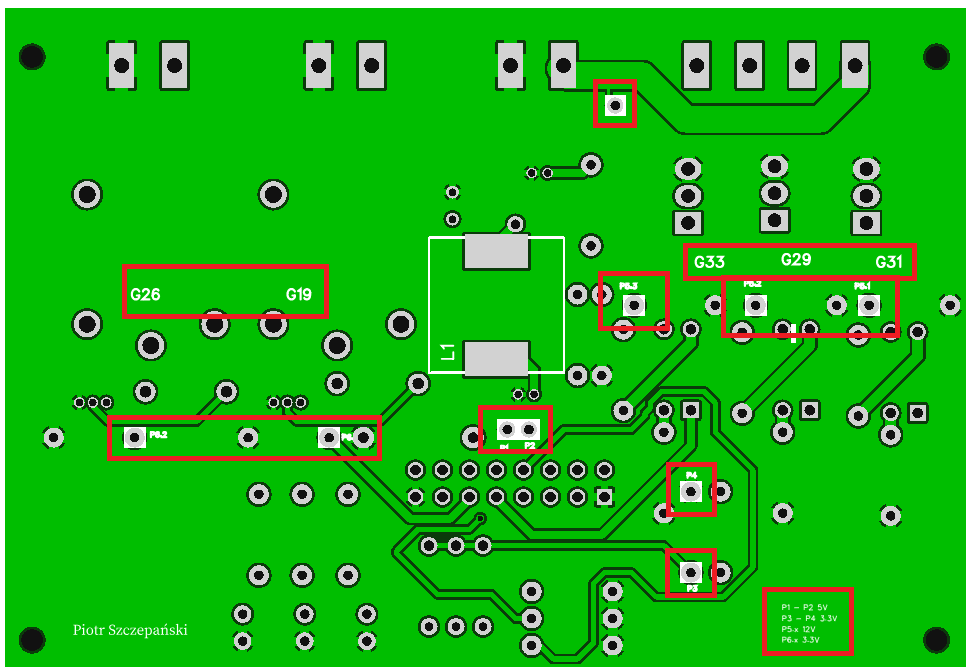
\includegraphics[width=0.6\textwidth]{pcb_dol_zaz.png}
                    \caption{Punkty kontroli poprawności działania}
                \end{center}
                \end{figure}
            Na płytce znajduje się, również oznaczenie mówiące o poprawnych wartościach między punktami kontrolnymi \emph{P1} - \emph{P4} oraz napięcia, które należy podać między masą a punktami \emph{P5} - \emph{P6}.
            Sprawdzenie poprawności montażu elemtów prztwronicy napięcia, odbywa się przez pomiar napięcia między punktami P1 P2, napięcie to powinnow wynosić 5V z xxx procentową dokładnością.
            Należy również sprawdzić wartość napięcia między punktami P3 P4, które powinno wynosić XXXXXX.
            W celu sprawdzenia sterownika paska LED należy podać 12V kolejno między masą, punktami P5.1, P5.2, P5.3 i mierzyć napięcie na odpowiadających wyjściach sterownika. Moduł działa poprawnie jeśli napięcie na wyjściu każdego z kanałów będzie równe 12V.
            Sprawdzeie wyjść przekaźnikowych odbywa się przez podnie 3.3V, z punktu P4, na punkty P6.1 i P6.2.
            Przekaźnik w momencie przełączania wydaje wyraźny dźwięk (kliknięcie), więc jego brak w chwili podłączenia napięcia oznacza niepoprawne działanie. Kolejnym etapem weryfikacji jest zmierzenie napięcia na wyjściach przekaźnikowych przy zwartych P6.1 lub P6.2 z P4, powinno ono być równe 12V.
            \\* Opisane metody testowania nie wymagają podłączenie Raspberry Pi, ale wymagają podłączenie zasilania 12V. 
            
            \subsubsection{Sprawdzenie poprawności działania całości modułu}
                \begin{figure}[H]
                \begin{center}
                    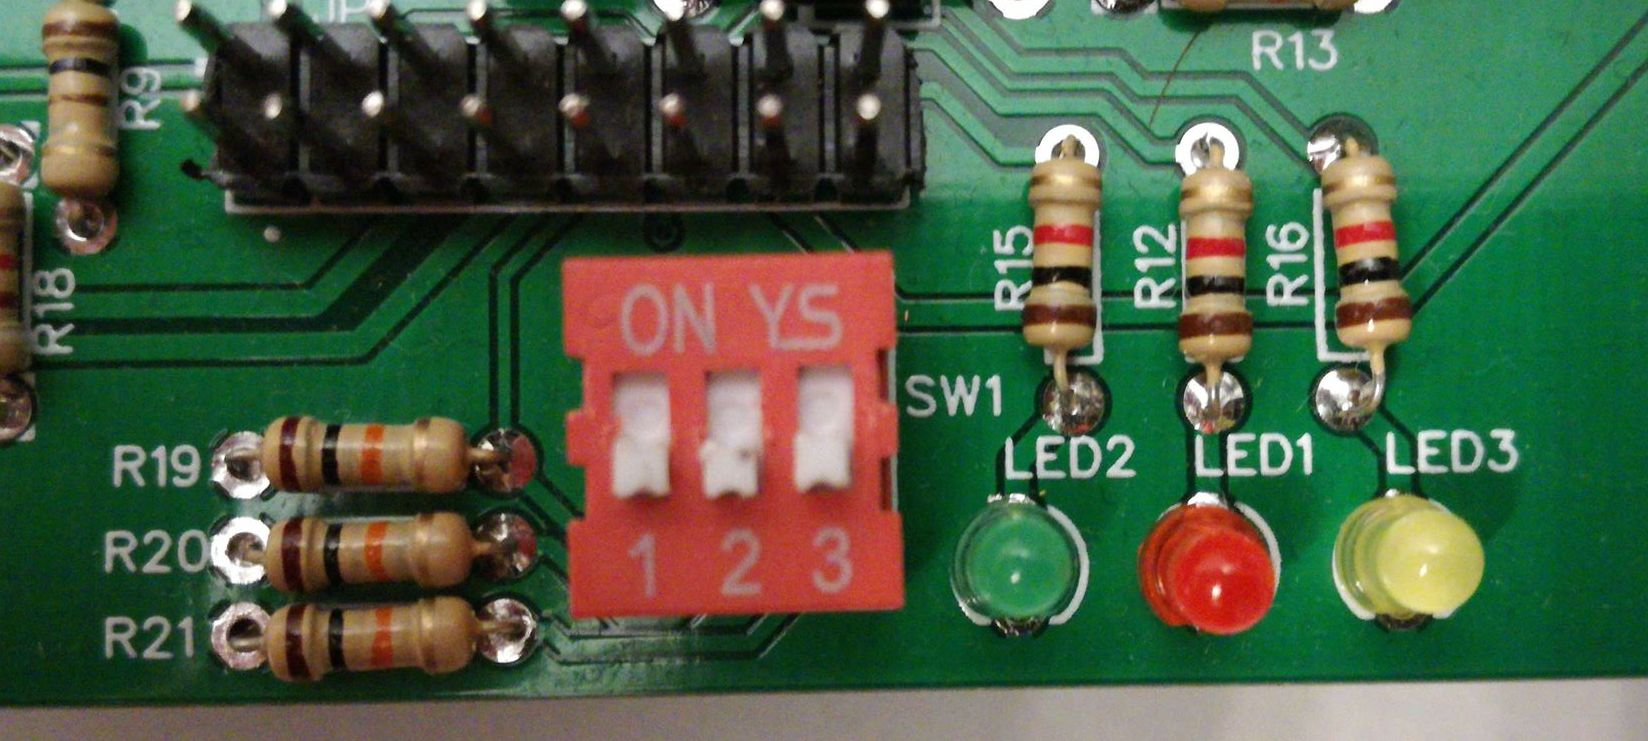
\includegraphics[width=0.5\textwidth]{dip_zoom.jpg}
                    \caption{Przełącznik trybów i diody sygnalizacyjne}
                \end{center}
                \end{figure}
            Sterownik udostępnia 3 tryby serwisowe wybierane za pomocą przełącznika suwakowego.
            Oprogramowanie sterownika odczytuje wartości, wejść do których podłączony jest przełącznik, w momencie startu systemu, więc aby włączyć tryb serwisowy należy odłączyć zasilanie modułu, wybrać tryb i podłączyć zasilanie. Nie jest dozwolnoe przełączenie dwóch lub więcej przełączników, w takim przypadku system zignoruje te informacje i uruchomi moduł w trybie pracy normalnej. Przejście modułu w tryb serwisowy sygnalizowane jest ciągłym podświetleniem diody \emph{LED3}.
            
            Dostępne tryby:
            \begin{itemize}
                \item przełącznik w pozycji 1 - w trybie tym sterownik będzie włączał i wyłączał z odstępem 1 sekundy wyjścia modułu w kolejnośc : kanał czerwony, kanał zielony, kanał niebieski, wyjście przekaźnikowe 1, wyjście przekaźnikowe 2. Tryb ten pozwala sprawdzić poprawność działania elektroniki wyjściowej oraz podłączenia modułu Raspberry Pi.
                
                \item przełącznik w pozycji 2 - tryb służy do sprawdzenia poprawności działania wyświetlacza, w szczególności poprawności wyświelania kolorów, czasu odświeżania dokładności powierzchni dotykowej.
                Na ekranie wyświeli się licznik inkrementujący swoją wartość od 0 do 10000 co 200ms, napis "TEST" w 3 rozmiarach oraz tło aplikacji będzie zmieniało kolory z częstotliwością 500ms w kolejności: czerwony, zielony, niebieski, biały. Ponadto na ekranie widoczne będą 4 pola dotykowe, których naciśnięcie będzie aktywowało diodę \emph{LED2}, w przypadku wykrycia dotyku poza, którymś z tych pól załączona zostanie dioda \emph{LED1}. 
                
                \item przełącznik w pozycji 3 - tryb służący do kontroli obciążenia procesora systemu, zajętości RAM-u oraz temperatury na procesorze. Informacje te będą wyświetlane na ekranie. Ponadto zostanie wyświelony plik kontrolny z poprzedniego uruchomienia modułu.
            \end{itemize}
            
            Wyłączenie trybu serwisowego jest możliwe dopiero po odłączniu zasilania i ustawieniu przełącznika serisowego do konfiguracji pracy standardowej.
            Moduł ignoruje zmiany przełącznika suwakowego w czasie działania programów.
            
            \newpage
            
            \section{Dokumentacja oprogramowania}
                \begin{figure}[H]
                \begin{center}
                    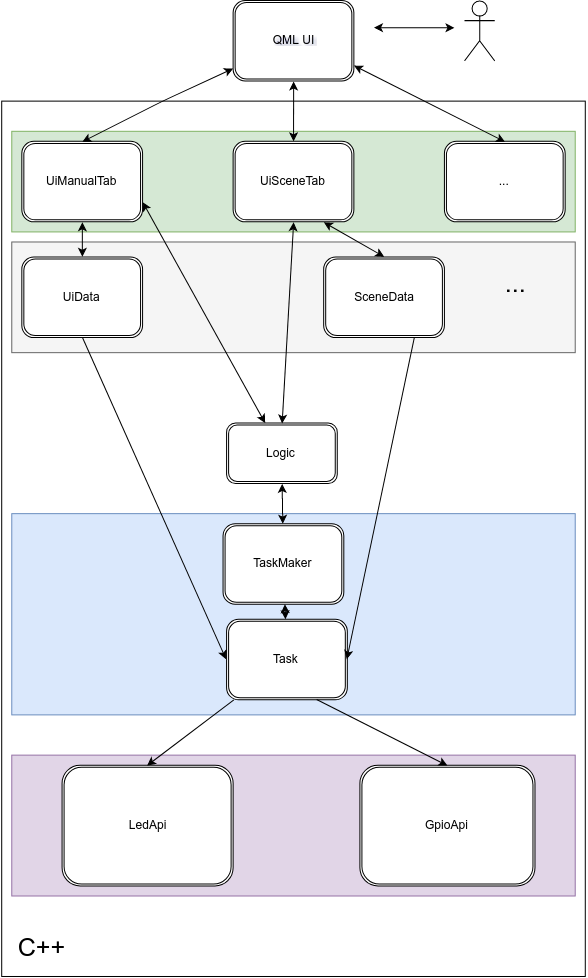
\includegraphics[width=0.5\textwidth]{inz_diag.png}
                    \caption{Schemat przepływu informacji w oprogramowaniu w trybie normalnego użytku}
                \end{center}
                \end{figure}
                \newpage
                
                \subsection{Interfejs graficzny}
                \subsection{}
                \newpage
                
                \subsection{Opis scenariuszy programowych}
                    \subsubsection{Start modułu}
                        \begin{figure}[H]
                        \begin{center}
                            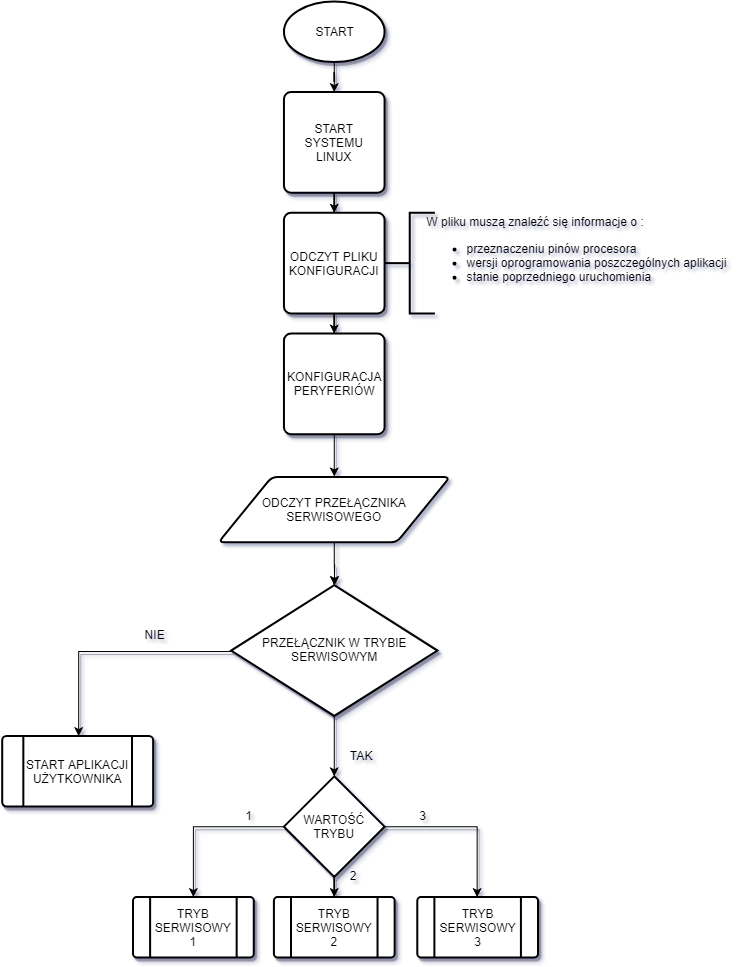
\includegraphics[width=0.7\textwidth]{startup.png}
                            \caption{Schemat blokowy startu modułu}
                        \end{center}
                        \end{figure}
                \subsection{Wykorzystane biblioteki}
                \subsection{}
            
\chapter{Wnioski i uwagi}
\thispagestyle{fancy}
  \cite{CleanCode,EffectiveModern,RpiBeginner}


% \listoffigures
% \listoftables
\bibliographystyle{plabbrv}

\addcontentsline{toc}{chapter}{Bibliografia} %utworzenie w spisie treści pozycji Bibliografia
\bibliography{bibliografia} % wstawia bibliografię korzystając z pliku bibliografia.bib - dotyczy BibTeXa, jeżeli nie korzystamy z BibTeXa należy użyć otoczenia thebibliography



\end{document}